\section{Einlesen}
\subsection{\fbox{read\_csv - read\_csv2}}
\textbf{Erzeugt Tibble}\\
\textbf{read\_csv}: Komma zum Zeilentrennen und Punkt für Dezimalzahlen\\
\textbf{read\_csv2}: Semicolon zum Zeilentrennen und Komma für Dezimalzahlen
\begin{rcode}{1]}
read_csv(file = "", col_types = "")
read_csv2(file = "", col_types = "")
\end{rcode}
Mit col\_types können wir als String wo jede Position für die jeweilige Spalten steht den Typ bestimmen\\
\textbf{Typen:}
\begin{itemize}[noitemsep]
  \item \textbf{c} = character
  \item \textbf{i} = integer
  \item \textbf{n} = number
  \item \textbf{d} = double
  \item \textbf{l} = logical
  \item \textbf{f} = factor
  \item \textbf{D} = date
  \item \textbf{T} = date time
  \item \textbf{t} = time
  \item \textbf{?} = guess
  \item \textbf{\_ oder -} = skip
\end{itemize}
\begin{rcode}{1]}
# Csv with ";" separator and "." as decimal point
read.csv("europe.data.csv", sep = ";", dec=".")

# Csv without first line as header
read.csv2("mpg.csv", header=F)

# Csv with 4 integer columns
read_csv2("magnets_pain.csv", col_types = "iiii")
\end{rcode}
\subsection{\fbox{read.csv - read.csv2}}
\textbf{Erzeugt Dataframe}
\begin{rcode}{1]}
data <- read.csv(file="", sep = ";", dec = ".") %>% as_tibble()
\end{rcode}
\begin{itemize}[noitemsep]
  \item \textbf{sep} = Das Zeichen welches die Spalten trennt.
  \item \textbf{dec} = Gibt den trenner für Dezimalzahlen an
\end{itemize}
\subsection{\fbox{read\_delim - read\_delim2}}
\textbf{Erzeugt Tibble}\\
Der Rest wie bei \_
\begin{rcode}{1]}
read_delim(file = , delim = ,col_types = "")
\end{rcode}
Mit der Option \textbf{delim} können wir festlegen, mit welchem Zeichen die Zeilen getrennt werden. 
\columnbreak
\subsection{\fbox{Tidy Data}}
\textbf{Typen:}
\begin{itemize}[noitemsep]
  \item Jede Spalte muss eine Variable sein
  \item Eine Observation ist eine Zeile
  \item Eine Variable ist z.B. das Alter
  \item Eine Observation ist "Jackson, 14"
\end{itemize}

\normalsize
\section{\fbox{Tidying Data}}
\subsection{\fbox{pivot\_longer()}}
\textbf{Wir haben eine Tabelle, wo es Spalten gibt, die als Variablen selber Observationen haben. Wir wollen diese Observationen auch als Observationen hinschreiben.}\\

\frame{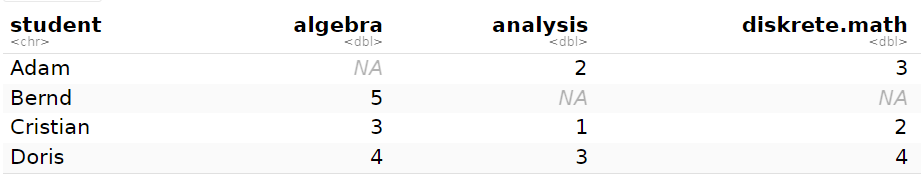
\includegraphics[draft=false, width=1\linewidth]{Figures/pivotlonger.png}}
Wir sehen, dass Algebra etc. eigentlich Observations sind.
\begin{rcode}{1]}
student1 %>% pivot_longer(cols =          algebra:diskrete.math, names_to = "classes", values_to = "grade", values_drop_na = T)
\end{rcode}
\begin{itemize}[noitemsep]
  \item \textbf{cols} = Ein c() mit allen Spalten oder spalte\_1 : spalte\_n.,
  \item \textbf{names\_to} = In welche Spalte die Namens aus cols.,
  \item \textbf{values\_to} = In welche Spalte die Werte die in den Spalten aus cols waren,
  \item \textbf{values\_drop\_na} = T falls wir NAs droppen wollen
\end{itemize}
\frame{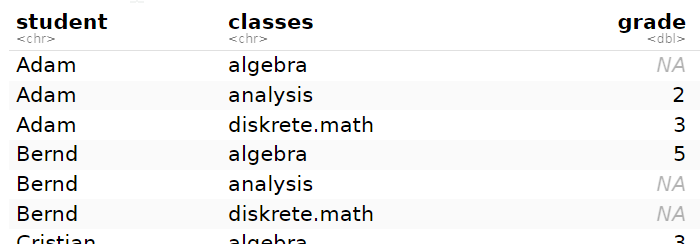
\includegraphics[draft=false, width=1\linewidth]{pivotlonger2.png}}
Hier haben wir jetzt in jeder Spalte eine Variable.
\columnbreak
\subsection{\fbox{pivot\_wider}}
Wir haben in einer Spalte für jede Observation zwei Variablen und in einer anderen Spalte die Observation für jede Variable.
\frame{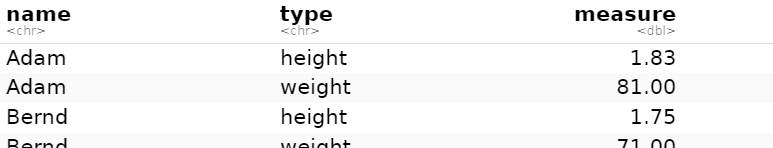
\includegraphics[draft=false, width=1\linewidth]{pivotwider.png}}
Jede Variable in Type soll eine eigene Spalte bekommen.
\begin{rcode}{1]}
student2 %>% pivot_wider(names_from = type, values_from = measure)
\end{rcode}
\begin{itemize}[noitemsep]
  \item \textbf{names\_from} = Die Spalte in der mehrere Variablen stehen.
  \item \textbf{values\_from} = Die Spalte wo die Werte drinnen stehen.
\end{itemize}
\frame{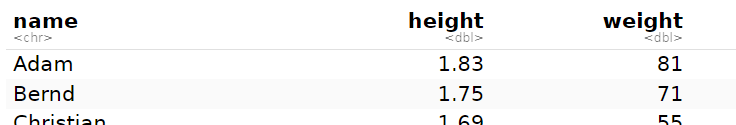
\includegraphics[draft=false, width=1\linewidth]{Figures/pivotwider2.png}}
Jetzt hat jede Variable eine Spalte
\section{\fbox{separate}}
Wir haben in einer Spalte zwei Werte in einer Zelle.
\frame{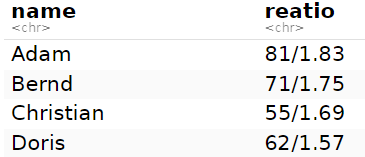
\includegraphics[draft=false, width=1\linewidth]{Figures/seperate.png}}
Nun wollen wir diese Spalte aufteilen.

\begin{rcode}{1}
student3 %>% separate(col = ratio, sep = "/", into = c("weight", " height"))
\end{rcode}
\begin{itemize}[noitemsep]
  \item \textbf{col} = Die Spalte in der die Observations sind. 
  \item \textbf{sep} = Das Zeichen, welches die Observations trennt.
  \item \textbf{into} = Spalten, in welche die Werte nun geschrieben werden sollen. 
  
  \textcolor{red}{WENN} Spalte unnötig 'NA': c(NA, "height")
  \item \textbf{convert} = True, wenn neue Spalten von char zu int umgewandelt werden sollen.
\end{itemize}
\frame{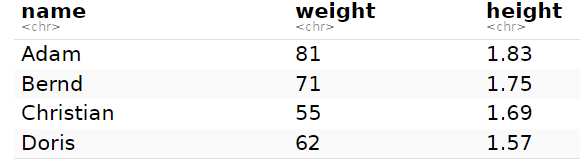
\includegraphics[draft=false, width=1\linewidth]{Figures/separate2.png}}

\columnbreak
\begin{markdown}
# Wichtige Befehle
## Anfang
knitr::opts_chunk$set(echo = TRUE, error = T)
- Global Options -> Code -> Editor - Keybindings -> Vim
- Global Options -> Code -> Display -> Rainbow Parentheses
- Für m und n in die Keybinds gehen und nach Operator suchen
### vim
imap jj \<Esc\>

## Libraries
{r include=F}

library(tidyverse)

library(TeachingDemos)

## Clean up code
- **STRG + i**

## Datenerzeugung
- **sample** = Erzeugt ein Sample aus den Werten in dem Array x mit der Länge size. Replace auf False wenn wir nur unique Werte aus x wollen.
- **runif** = Ein Array mit Länge n mit Werten von min bis max.
```R
df <- tibble(
  id = 1:10,
  sex = sample(x = c("f", "m"),
    size = 10, 
    replace = T),
  age = round(runif(n = 10, min = 10, max = 35)),
)
```

## Tibble Zeugs
### Zeile Löschen
```R
df %>% '['(-1,)
```
### filtern
- **filter** = Kann ich nach Werten filtern.
- **%in%** = falls ich mehrere Sachen in einer Variable filtern will.
```R
students %>% 
  filter(sex == "m")
flights %>% 
  filter(carrier %in% c("AA", "DL"))
flights %>% 
  filter(carrier == "AA" | carrier == "DL")
```
### NA Werte filtern
- **!is.na(Zeile)** = Entfernt uns alle NA Werte
```R
corona %>% filter(!is.na(new_cases))
```
### select
- **select** = ich kann einzelne Spalten auswählen
```R
students %>% select(age)
```
### Zeile hinzufügen
- **add_row** = wir müssen jeden Wert explizit angeben.
```R
students %>% add_row(
    id = 11,
    sex = "m", 
    age = 25, 
    score1 = 4
)
```
### Werte in Kategorien
```R
df <- df %>% mutate(
  grade = case_when(
    sum <= 37 ~ 5,
    sum > 37 & sum <= 45 ~ 4,
    sum > 35 & sum <= 55 ~ 3,
    sum > 55 & sum <= 65 ~ 2,
    sum > 65 ~ 1))
```
### ifelse
```R
mutate(
  passed = ifelse(grade < 5, yes = 1, no = 0)
)
```
### Werte sortieren
- **arrange** = Wir sortieren den Tibble nach der ausgewählten Spalte. Wenn andersherum die Spalte mit desc() umgeben.
```R
df %>% select(id, sex , grade) %>% 
  arrange(sex) 
# oder 
  arrange(desc(sex))
```

### Summarise
- **summarise** = Erstellt eine Übersichtstabelle die nur die Spalten beschreibt die ich angebe, die Spalte nach der ich groupe und die, die ich angebe.
- **quantile** - gibt mir die Quantile erst die Spalte dann welches quantile
```R
**Interquartile** = Q3 - Q1
df %>% group_by(sex) %>% 
  summarise(mean_score = mean(sum),
            min_score = min(sum),
            max_score = max(sum),
            med_score = median(sum),
            sd_score = sd(sum),
            Q1 = quantile(sum, 0.25),
            Q2 = quantile(sum, 0.5),
            Q3 = quantile(sum, 0.75),
            IQR = Q3 - Q1
            )
```
### Trimmed Mean
- **trim** <- Wenn ich einen Trimmed Mean 40% habe, schneide ich jeweils 20% der kleinsten und größten Werte weg
```R
mean(observations, trim = 0.2)
```
### Geometric Mean
```R
exp(mean(log(x)))
```
### Coefficient of Variation
```R
sd(x) / mean(x)
```
### Werte zählen
- **n** <- um n() benutzen zu können, muss ich summarise benutzen.
- **count** <-  count() kann ich immer benutzen, muss aber die Spalte explizit angeben.
```R
er %>% group_by(group) %>% 
  summarise(n = n())
er %>% count(group)
```
### Rowwise
- **rowwise()** <- Macht dasselbe wie ein group_by für jede Zeile.
```R
er %>% rowwise() %>% 
  mutate(x = sum(ex1:ex5))
```
- Ohne Rowwise <- Berechnet die Summe aller Spalten ex für alle Zeilen.

- Mit Rowwise <- Berechnet jeweils die Summe für jede einzelne Zeile.

### Unique
- **unique** = Wenn ich alle unique Zeilen zeigen will. 

Gut kombinierbar mit select.

### Determine number and rates of Variables

```R
data.fail <- data.grade %>% 
    group_by(subject, attempt) %>% 
    mutate(
        failed = ifelse(grade == 5, 1, 0)
    ) %>% 
    summarise(
        no = n(),
        ratio = sum(failed) / no
    )
```

### Die obersten n Werte
```R
df %>% head(10)
```
# Diagramme und so ein Mist
## plot - Standard ist Scatterplot
Im Normalfall einfach x und y reinwerfen
- **type** - "l" gibt uns einen Lineplot. In ?plot stehen die anderen Optionen.
```R
plot(x = x_werte, y = y_werte, type = "l")
```

## Boxplot
### Tilde - y ~ x
In y stehen die Werte.
Ich ordne die Werte dem jeweiligen Typen in x zu
```R
boxplot(y ~ x)
boxplot(werte ~ typen)
boxplot(data$score ~ data$attempt)
```
Die linke Variable ist in Abhängigkeit der rechten Variable.

### Skewness
- Right Skewed <- Wenn der rechts/obere Whisker länger ODER Median niedrig in der Box
- Left Skewed <- Wenn der linke/untere Whisker länger ODER Median hoch in der Box
- Symmetrisch <- Wenn Median mittig UND Whiskers gleich lang

## Pie Chart - Kuchendiagramm
- **labels** - Die Beschreibung für jedes Kuchenstück
- **col** - Die Farben
```R
pie(party$Results_2013,
    labels  = party$Party,
    col = party$colors)
```
## Barplot - Balkendiagramm
- **names.arg** - Name
- **col** - Farben :)
```R
barplot(party$Results_2013,
        names.arg = results$Party,
        col = results$colors)
```
# Cumulative Frequency Distribution
Selbe Idee wie pnorm. 

Also h(700) sagt uns wie viele der Werte unter 700 liegen.
- **ecdf** 
```R
h <- ecdf(data)
plot(h)
```
### less equal 800
```R
h(800)
```
### greater than 725
```R
1 - h(725)
```
### greater than 642 und less equal 777
```R
h(777) - h(642)
```
### equal 696
```R
h(697) - h(695)
```
# Linear Regression
## Scatterplot
```R
plot(x, y)
```
## Covariance
Die Kovarianz misst den Grad, zu dem zwei Zufallsvariablen gemeinsam variieren
```R
cov(x, y)
```
## Coefficient of Correlation
Ist dasselbe wie Covarianz aber genormt. 
Zeigt wie stark zwei Variablen zusammenhängen. 

- 1 -> steigen perfekt zusammen 
- -1 -> fallen perfekt zusammen
- 0 -> bedeutet kein Zusammenhang
```R
cor(x, y)
```
## Coefficient of Determination = Proportion of Variation
Tells you how your model or line explains your data.
- 1 -> your model explains 100% of your data
- 0.5 -> your model explains 50% of your data
- 0 -> your model is useless just like you
```R
cor(x, y)^2
```
## Regression line Y ~ X
- Criterion is our Y 
- Predictor is our X
- a ist unser y-Achsenabschitt/Intercept
- b ist unsere Steigung/Slope
### abline zeichnet unsere Linie
Wir müssen als erstes Plotten.


**In RMarkdown für abline den ganzen Codeblock ausführen.**
```R
plot(x, y)
model <- lm(y ~ x)
abline(model)
```
### a und b bekommen
 y = a + b * x 
```R
model <- lm(y ~ x)
a <- model$coefficients[1]
b <- model$coefficients[2]
```
### Predict value for x = 8
```R
model <- lm(y ~ x)
a <- model$coefficients[1]
b <- model$coefficients[2]
new_y <- a + b * 8
```
## Regression line X ~ Y
```R
- Criterion is our X
- Predictor is our Y
xy_model <- lm(x ~ y)
alpha <- xy_model$coefficients[1]
beta <- xy_model$coefficients[2]
a_line <- -(alpha / beta)
b_line <- 1 / beta
abline(a = a_line, b = b_line, col = "red")
```

# Contingency table

## Mit 2 Spalten x \& y

```R
chisq.test(x, y)
```

## Keyword: Contingency Table - Observed Values
```R
chisq.test(x, y)$observed
```

## Keyword: Indifference Table - Expected values
```R
chisq.test(tab)$expected
```
## X hoch 2
```R
x2 <- chisq.test(x, y)$statistic
```
## C
```R
c <- sqrt((x2 / (x2 + sum(tab))))
```
## C corr
```R
c_korr <- sqrt((min(length, height)/(min(length, height) -1)) * x2/(x2+sum(tab)))
```
- 0.0-0.3 <- Keine Assoziation
- 0.3-0.8 <- Some kind of Assoziation
- 0.8-1.0 <- Strong Assoziation

## Mit Matrix

40 | 10 | 50

20 | 10 | 30

10 | 10 | 20

70 | 30 | 100


Wir müssen nicht die gesamt Felder betrachten
- **nrow** - wie viele Zeilen wir haben
- **ncol** - wie viele spalten wir haben
Die daten werden automatisch eingeordnet
```R
tab <- matrix(c(40, 10, 20, 10, 10, 10), 
    nrow = 3, 
    ncol = 2, 
    byrow = T)

chisq.test(tab)
```

## Spearman Rank Correlation

```R
cor.test(x, y, method = "spearman")
```

## Conditional Relative Frequency Distribution

```R
tab / rowSums(tab)
```

# R shenanigans
## groups fehlermeldung muten
```R
summarize(.groups = "drop")
```
### Ganzzahldivision
```R
x %/% y
```
### Modulo ( x mod y)
```R
x %% y
```

\end{markdown}

\newpage

\textbf{Qualitative, Nominal, Discrete}
\begin{itemize}
    \item Gender
    \item Religion
    \item Course
    \item Exam
    \item Country
    \item Color
    \item Binary yes/no question
    \item Name
    \item Hair color
    \item Type of Transmission
    \item Type of Train
    \item Fuel Type
    \item Immatriculation Number
\end{itemize}

\textbf{Quantitative, Ordinal, Discrete}
\begin{itemize}
    \item Score (when multiple exams in column)
    \item Marks in Maths
    \item Rating of Movie on 7-Point
    \item Attitude towards something
\end{itemize}




\textbf{Quantitative, Interval, Discrete}
\begin{itemize}
    \item Birthday
    \item IQ
    \item Year
    \item Month
    \item Day
\end{itemize}

\textbf{Quantitative, Interval, Continuous}
\begin{itemize}
    \item Temperature in Celsius/Fahrenheit
\end{itemize}

\textbf{Quantitative, Ratio, Discrete}
\begin{itemize}
    \item Age
    \item Population
    \item Attempt
    \item Semester
    \item Credit Points
    \item Number of bottles of wine
    \item Number of Cylinders
\end{itemize}

\columnbreak

\textbf{Quantitative, Ratio, Continuous}
\begin{itemize}
    \item Height
    \item Weight
    \item Size
    \item Time to respond
    \item Engine Displacement in Litre
    \item Miles per Gallon
    \item Temperature in Kelvin
    \item BMI
\end{itemize}

\textbf{Quantitative, Ratio, Discrete (Special Case)}
\begin{itemize}
    \item Score (when one exam in column)
\end{itemize}

\section{Variables}

\subsection{Type}

- Qualitative <- Bedeutet Kategorien.

- Quantitative <- Bedeutet messbar bzw. abzählbar.

\subsection{Scale}

- Nominal <- Daten sind in unique Kategorien: 

blau, braun, grün

- Ordinal <- Daten können gerankt werden: 

gut, mittel, schlecht

- Interval <- Daten haben selbes Intervall aber keinen absoluten Nullpunkt: 

Celsius

- Ratio <- Daten haben absoluten Nullpunkt, dadurch ist auch das doppelte eines Wertes wirklich das doppelte: 

Kelvin

\subsection{Range}

- Discrete <- Bedeutet endlich.

- Continuous <- Bedeutet unendlich viele Werte zwischen zwei Werten.

